%==============================================================================
% tento soubor pouzijte jako zaklad
% this file should be used as a base for the thesis
% Autoři / Authors: 2008 Michal Bidlo, 2018 Jaroslav Dytrych
% Kontakt pro dotazy a připomínky: dytrych@fit.vutbr.cz
% Contact for questions and comments: dytrych@fit.vutbr.cz
%==============================================================================
% kodovani: UTF-8 (zmena prikazem iconv, recode nebo cstocs)
% encoding: UTF-8 (you can change it by command iconv, recode or cstocs)
%------------------------------------------------------------------------------
% zpracování / processing: make, make pdf, make clean
%==============================================================================
% Soubory, které je nutné upravit: / Files which have to be edited:
%   projekt-20-literatura-bibliography.bib - literatura / bibliography
%   projekt-01-kapitoly-chapters.tex - obsah práce / the thesis content
%   projekt-30-prilohy-appendices.tex - přílohy / appendices
%==============================================================================
%\documentclass[]{fitthesis} % bez zadání - pro začátek práce, aby nebyl problém s překladem
%\documentclass[english]{fitthesis} % without assignment - for the work start to avoid compilation problem
%\documentclass[zadani]{fitthesis} % odevzdani do wisu a/nebo tisk s barevnými odkazy - odkazy jsou barevné
%\documentclass[english,zadani]{fitthesis} % for submission to the IS FIT and/or print with color links - links are color
%\documentclass[zadani,print]{fitthesis} % pro černobílý tisk - odkazy jsou černé
%\documentclass[english,zadani,print]{fitthesis} % for the black and white print - links are black
\documentclass[zadani,cprint]{fitthesis} % pro barevný tisk - odkazy jsou černé, znak VUT barevný
%\documentclass[english,zadani,cprint]{fitthesis} % for the print - links are black, logo is color
% * Je-li práce psaná v anglickém jazyce, je zapotřebí u třídy použít 
%   parametr english následovně:
%   If thesis is written in english, it is necessary to use 
%   parameter english as follows:
%      \documentclass[english]{fitthesis}
% * Je-li práce psaná ve slovenském jazyce, je zapotřebí u třídy použít 
%   parametr slovak následovně:
%   If the work is written in the Slovak language, it is necessary 
%   to use parameter slovak as follows:
%      \documentclass[slovak]{fitthesis}
% * Je-li práce psaná v anglickém jazyce se slovenským abstraktem apod., 
%   je zapotřebí u třídy použít parametry english a enslovak následovně:
%   If the work is written in English with the Slovak abstract, etc., 
%   it is necessary to use parameters english and enslovak as follows:
%      \documentclass[english,enslovak]{fitthesis}

% Základní balíčky jsou dole v souboru šablony fitthesis.cls
% Basic packages are at the bottom of template file fitthesis.cls
% zde můžeme vložit vlastní balíčky / you can place own packages here

% Kompilace po částech (rychlejší, ale v náhledu nemusí být vše aktuální)
% Compilation piecewise (faster, but not all parts in preview will be up-to-date)
% \usepackage{subfiles}

% Nastavení cesty k obrázkům
% Setting of a path to the pictures
%\graphicspath{{obrazky-figures/}{./obrazky-figures/}}
%\graphicspath{{obrazky-figures/}{../obrazky-figures/}}

%---rm---------------
\renewcommand{\rmdefault}{lmr}%zavede Latin Modern Roman jako rm / set Latin Modern Roman as rm
%---sf---------------
\renewcommand{\sfdefault}{qhv}%zavede TeX Gyre Heros jako sf
%---tt------------
\renewcommand{\ttdefault}{lmtt}% zavede Latin Modern tt jako tt

% vypne funkci šablony, která automaticky nahrazuje uvozovky,
% aby nebyly prováděny nevhodné náhrady v popisech API apod.
% disables function of the template which replaces quotation marks
% to avoid unnecessary replacements in the API descriptions etc.
\csdoublequotesoff

% =======================================================================
% balíček "hyperref" vytváří klikací odkazy v pdf, pokud tedy použijeme pdflatex
% problém je, že balíček hyperref musí být uveden jako poslední, takže nemůže
% být v šabloně
% "hyperref" package create clickable links in pdf if you are using pdflatex.
% Problem is that this package have to be introduced as the last one so it 
% can not be placed in the template file.
\ifWis
\ifx\pdfoutput\undefined % nejedeme pod pdflatexem / we are not using pdflatex
\else
  \usepackage{color}
  \usepackage[unicode,colorlinks,hyperindex,plainpages=false,pdftex]{hyperref}
  \definecolor{hrcolor-ref}{RGB}{223,52,30}
  \definecolor{hrcolor-cite}{HTML}{2F8F00}
  \definecolor{hrcolor-urls}{HTML}{092EAB}
  \hypersetup{
	linkcolor=hrcolor-ref,
	citecolor=hrcolor-cite,
	filecolor=magenta,
	urlcolor=hrcolor-urls
  }
  \def\pdfBorderAttrs{/Border [0 0 0] }  % bez okrajů kolem odkazů / without margins around links
  \pdfcompresslevel=9
\fi
\else % pro tisk budou odkazy, na které se dá klikat, černé / for the print clickable links will be black
\ifx\pdfoutput\undefined % nejedeme pod pdflatexem / we are not using pdflatex
\else
  \usepackage{color}
  \usepackage[unicode,colorlinks,hyperindex,plainpages=false,pdftex,urlcolor=black,linkcolor=black,citecolor=black]{hyperref}
  \definecolor{links}{rgb}{0,0,0}
  \definecolor{anchors}{rgb}{0,0,0}
  \def\AnchorColor{anchors}
  \def\LinkColor{links}
  \def\pdfBorderAttrs{/Border [0 0 0] } % bez okrajů kolem odkazů / without margins around links
  \pdfcompresslevel=9
\fi
\fi
% Řešení problému, kdy klikací odkazy na obrázky vedou za obrázek
% This solves the problems with links which leads after the picture
\usepackage[all]{hypcap}

% Informace o práci/projektu / Information about the thesis
%---------------------------------------------------------------------------
\projectinfo{
  %Prace / Thesis
  project={BP},            %typ práce BP/SP/DP/DR  / thesis type (SP = term project)
  year={2019},             % rok odevzdání / year of submission
  date=\today,             % datum odevzdání / submission date
  %Nazev prace / thesis title
  title.cs={Bezpečnostní analýza karet Mifare Classic},  % název práce v češtině či slovenštině (dle zadání) / thesis title in czech language (according to assignment)
  title.en={Security Analysis of Mifare Classic Smart Cards}, % název práce v angličtině / thesis title in english
  %title.length={14.5cm}, % nastavení délky bloku s titulkem pro úpravu zalomení řádku (lze definovat zde nebo níže) / setting the length of a block with a thesis title for adjusting a line break (can be defined here or below)
  %Autor / Author
  author.name={Martin},   % jméno autora / author name
  author.surname={Bobčík},   % příjmení autora / author surname 
  %author.title.p={Bc.}, % titul před jménem (nepovinné) / title before the name (optional)
  %author.title.a={Ph.D.}, % titul za jménem (nepovinné) / title after the name (optional)
  %Ustav / Department
  department={UITS}, % doplňte příslušnou zkratku dle ústavu na zadání: UPSY/UIFS/UITS/UPGM / fill in appropriate abbreviation of the department according to assignment: UPSY/UIFS/UITS/UPGM
  % Školitel / supervisor
  supervisor.name={Ondřej},   % jméno školitele / supervisor name 
  supervisor.surname={Hujňák},   % příjmení školitele / supervisor surname
  supervisor.title.p={Ing.},   %titul před jménem (nepovinné) / title before the name (optional)
  supervisor.title.a={},    %titul za jménem (nepovinné) / title after the name (optional)
  % Klíčová slova / keywords
  keywords.cs={RFID technologie, chytré karty, bezkontaktní karty, MIFARE Classic, šifra CRYPTO1, zranitelnosti, Chameleon Mini, emulace karet, relay útok, kryptoanalýza, C\# .Net}, % klíčová slova v českém či slovenském jazyce / keywords in czech or slovak language
  keywords.en={RFID technology, smart cards, contactless cards, MIFARE Classic, CRYPTO1 cipher, vunerabilities, Chameleon Mini, card emulation, relay attack, cryptoanalysis, C\# .Net}, % klíčová slova v anglickém jazyce / keywords in english
  %keywords.en={Here, individual keywords separated by commas will be written in English.},
  % Abstrakt / Abstract
  abstract.cs={Cílem této bakalářské práce je studium bezpečnosti chytrých, bezkontaktních karet MIFARE Classic a analýza rizik spojených s jejich využíváním. Popisuje jednotlivé známé zranitelnosti v návrhu těchto karet a jejich šifrovacího algoritmu CRYPTO1. V této práci je dále experimentováno se zařízením Chameleon Mini, s jehož pomocí jsou provedeny dva útoky a jedna kryptoanalýza karty. Konkrétně emulace karty, relay útok a analýza nedostatečné náhodnosti generátoru pseudonáhodných čísel karty. Z těchto se úspěšně podařila pouze emulace karet.}, % abstrakt v českém či slovenském jazyce / abstract in czech or slovak language
  abstract.en={Goal of this bachelor thesis is a security study of MIFARE Classic contactless smart cards and risk analysis of their usage. There are described individual vunerabilities in the design and CRYPTO1 cipher of such cards. In this thesis is also experimented with Chameleon Mini device, which is used to perform two attacks and one cryptoanalysis of the cards. Namely, card emulation, relay attack, and analysis of insufficient randomness of cards' pseudorandom number generator. From those, only card emulation was fully successful. }, % abstrakt v anglickém jazyce / abstract in english
  %abstract.en={An abstract of the work in English will be written in this paragraph.},
  % Prohlášení (u anglicky psané práce anglicky, u slovensky psané práce slovensky) / Declaration (for thesis in english should be in english)
  declaration={Prohlašuji, že jsem tuto bakalářskou práci vypracoval samostatně pod vedením pana Ing.~Ondřeje Hujňáka.
Uvedl jsem všechny literární prameny a publikace, ze kterých jsem čerpal.},
  %declaration={Hereby I declare that this bachelor's thesis was prepared as an original author’s work under the supervision of Mr. X
% The supplementary information was provided by Mr. Y
% All the relevant information sources, which were used during preparation of this thesis, are properly cited and included in the list of references.},
  % Poděkování (nepovinné, nejlépe v jazyce práce) / Acknowledgement (optional, ideally in the language of the thesis)
  acknowledgment={Tímto bych velmi rád poděkoval Ing. Ondřeji Hujňákovi za poskytnutý čas, cenné rady a odborné vedení při řešení této práce.},
  %acknowledgment={Here it is possible to express thanks to the supervisor and to the people which provided professional help
%(external submitter, consultant, etc.).},
  % Rozšířený abstrakt (cca 3 normostrany) - lze definovat zde nebo níže / Extended abstract (approximately 3 standard pages) - can be defined here or below
  %extendedabstract={Do tohoto odstavce bude zapsán rozšířený výtah (abstrakt) práce v českém (slovenském) jazyce.},
  %faculty={FIT}, % FIT/FEKT/FSI/FA/FCH/FP/FAST/FAVU/USI/DEF
  faculty.cs={Fakulta informačních technologií}, % Fakulta v češtině - pro využití této položky výše zvolte fakultu DEF / Faculty in Czech - for use of this entry select DEF above
  faculty.en={Faculty of Information Technology}, % Fakulta v angličtině - pro využití této položky výše zvolte fakultu DEF / Faculty in English - for use of this entry select DEF above
  department.cs={Ústav matematiky}, % Ústav v češtině - pro využití této položky výše zvolte ústav DEF nebo jej zakomentujte / Department in Czech - for use of this entry select DEF above or comment it out
  department.en={Institute of Mathematics} % Ústav v angličtině - pro využití této položky výše zvolte ústav DEF nebo jej zakomentujte / Department in English - for use of this entry select DEF above or comment it out
}

% Rozšířený abstrakt (cca 3 normostrany) - lze definovat zde nebo výše / Extended abstract (approximately 3 standard pages) - can be defined here or above
%\extendedabstract{Do tohoto odstavce bude zapsán výtah (abstrakt) práce v českém (slovenském) jazyce.}

% nastavení délky bloku s titulkem pro úpravu zalomení řádku - lze definovat zde nebo výše / setting the length of a block with a thesis title for adjusting a line break - can be defined here or above
%\titlelength{14.5cm}


% řeší první/poslední řádek odstavce na předchozí/následující stránce
% solves first/last row of the paragraph on the previous/next page
\clubpenalty=10000
\widowpenalty=10000

% checklist
\newlist{checklist}{itemize}{1}
\setlist[checklist]{label=$\square$}

\begin{document}
  % Vysazeni titulnich stran / Typesetting of the title pages
  % ----------------------------------------------
  \maketitle
  % Obsah
  % ----------------------------------------------
  \setlength{\parskip}{0pt}

  {\hypersetup{hidelinks}\tableofcontents}
  
  % Seznam obrazku a tabulek (pokud prace obsahuje velke mnozstvi obrazku, tak se to hodi)
  % List of figures and list of tables (if the thesis contains a lot of pictures, it is good)
  \ifczech
    \renewcommand\listfigurename{Seznam obrázků}
  \fi
  \ifslovak
    \renewcommand\listfigurename{Zoznam obrázkov}
  \fi
  % \listoffigures
  
  \ifczech
    \renewcommand\listtablename{Seznam tabulek}
  \fi
  \ifslovak
    \renewcommand\listtablename{Zoznam tabuliek}
  \fi
  % \listoftables 

  \ifODSAZ
    \setlength{\parskip}{0.5\bigskipamount}
  \else
    \setlength{\parskip}{0pt}
  \fi

  % vynechani stranky v oboustrannem rezimu
  % Skip the page in the two-sided mode
  \iftwoside
    \cleardoublepage
  \fi

  % Text prace / Thesis text
  % ----------------------------------------------
  %===============================================================================

%                                   NADPIS                      
\chapter{Úvod}
\label{uvod}


%                                   NADPIS                      
\chapter{Radio frekvenční identifikace}
\label{technologie_rfid}
V této kapitole jsou popsány principy komunikace pomocí radio frekvenční identifikace (dále jen~RFID), její historie, jednotlivé komponenty a využití v průmyslu a každodenním životě.

\section{Úvod do RFID}
RFID je zkratka pro {Radio-Frequency IDentification}, tedy identifikace pomocí rádiové frekvence (dále jen~RF). Tato technologie umožňuje bezdrátovou komunikaci na relativně krátkou vzdálenost\cite{The_RF_in_RFID}.
\par
RFID a bezdrátové technologie \cite{Smart_Cards_Tokens_Security}{ - str.321-347}

\section{Historie}
%\subsection{Čárové kódy}
Principy~RFID byly poprvé použity v systému~IFF (Identity: Friend or Foe) za 2. světové války Britskou armádou. Tento systém měl za úkol rozlišit vlastní letadla od nepřátelských. Proto byla vybavena nastavitelným {radio-majákem}, který byl schopen vysílat 6~identifikačních kódů. Systém pracoval v principu tak, že vysílač (radar) vyslal dotaz směrem k letadlu. Po dosažení a zpracování signálu odpovídač (transpondér) na letadle vyslal signál zpět, čímž došlo k zjištění příslušnosti stroje. Transpondér mohl odpovídat dvěma způsoby. Pasivní systém využil odražený původní signál a upravil ho tak aby obsahoval potřebné informace. Tento princip je dnes nejvíce využívaným způsobem identifikace pomocí RFID. Naopak aktivní systém přijal signál a sám okamžitě odeslal odpověď,přičemž ta mohla být odeslána i na jiné nosné frekvenci. V padesátých letech minulého století se radio identifikace rozmohla z armády do celého letectví a používá se dodnes. %\cite{The_RF_in_RFID}\cite{Emulator_UHD_RFID_Tagu}.
\par
RFID vznikla jako alternativa k čárovým kódům. I když je výroba čárových kódů levnější, mají proti RFID mnoho nevýhod. Pro čtení musí čtecí zařízení přímo vidět na štítek s kódem. Nesmí být snížená jeho vizuální čitelnost, například špínou, popisovačem, nebo pokroucením. Zápis více informací se dá řešit pouze zvětšením plochy štítku, nebo použitím jemnějšího značení, které je ale viditelné z menší vzdálenosti. Modifikace dat uložených pomocí čárových kódů se dá prakticky řešit pouze tiskem nového kódu \cite{The_RF_in_RFID}\cite{Emulator_UHD_RFID_Tagu}.

\section{Tagy}
Primární využití RFID tagů spočívá v identifikaci objektů. Cena takových objektů je nesrovnatelně vyšší oproti ceně tagu. Pokud je značený objekt levný, tag musí být ještě levnější. Na rozdíl od RFID~čteček jsou tagy prakticky pořád v pohybu, ať už jako chytré karty, nebo identifikátory zboží, vlaků kontejnerů apod. Tagy tedy musí být velmi levné za vysoké odolnosti proti fyzickému poškození\cite{The_RF_in_RFID}.
RFID~tag je systém skládající se minimálně z mikročipu, antény a pouzdra. Mikročip obsahuje pamět a logické obvody pro příjímání a odesílání dat čtecímu zařízení. Anténa přijímá signál z čtečky a poté jej zpětně rozptýlí (dále jen backscatter modulace) odesílanými daty. Pouzdro je potřeba pro udržení integrity tagu a jako ochrana proti vnějšímu poškození samotného čipu a antény\cite{RFID_explained}.
RFID tagy se dělí na aktivní, pasivní a částečně pasivní podle toho zda je jsou napájeny z externího, nebo interního zdroje\cite{The_RF_in_RFID}. Rozdíl je také v tom, kdo iniciuje komunikaci. Aktivní tag komunikaci zahajuje sám, zatímco komunikaci s pasivními tagy musí zahájit sama čtečka\cite{Hazardous_areas}. 

\subsection{Pasivní tagy}
Pasivní tagy identifikují levné objekty. Interní zdroj, i ve formě malé baterie, je pro ně příliš velký a drahý. Stejně jako transmittery a příjímače používané v klasických radiových zařízeních. Bez konvenčního zdroje energie jsou prakticky použitelné pouze jednoduché obvody, které je možno napájet bezdrátově i na vzdálenost několika metrů od čtecího zařízení. 
\par 
Aby mohl integrovaný obvod tagu pracovat potřebuje zdroj stejnosměrného proudu několika desítek mikroampérů o napětí  jeden až tři volty v závislosti na typu použitých tranzistorů. Toto napětí musí tag získat z RF signálu\cite{The_RF_in_RFID}. Frekvence tohoto signálu se podle použití liší. Od použité frekvence se také odvíjí dosah čtení a rychlost přenosu dat. Používané frekvence spadají do několika pásem, a a to nízká frekvence ({Low Frequency - LF}), vysoká frekvence ({High Frequency - HF}) a ultra vysoká frekvence ({Ultra High Frequency - UHF}). Evropská a americká specifikace pásma~UHF se liší ve frekvenci(viz. tabulka \ref{tabulka_pasem}). Chytré karty používají HF~pásmo\cite{Smart_Cards_Tokens_Security}. 

\begin{table}[]
\begin{tabular}{cccc}
\hline
Pásmo               & Frekvence   & Dosah   & Přenosová rychlost \\ \hline
LF                  & 125-135 kHz & 1-2 m   & 100 bps            \\
HF                  & 13,56 MHz   & 2 m     & 2 kbps             \\
UHF-Evropa          & 865-868 MHz & 12-20 m & 40-640 kbps        \\
UHF-Severní Amerika & 902-928 MHz & 12-20 m & 40-640 kbps        \\ \hline
\end{tabular}
\caption{Porovnání vlastností operačních pásem RFID\cite{RFID_explained}\cite{The_RF_in_RFID}}
\label{tabulka_pasem}
\end{table}

\subsection{Aktivní tagy} %\par ?? 
Aktivní tagy jsou napájeny z vlastního zdroje. Ten může být buď baterie, nebo připojení do elektrické infrastruktury. Zdroj napájí nejenom přenos dat, ale i ostatní elektronické komponenty. Těmito komponentami mohou být různé senzory nebo uživatelské rozhraní\cite{RFID_explained}. Vzhledem k technologii logických obvodů postupuje vývoj baterií velmi pomalu. Jedním z hlavních problémů návrhu těchto tagů je tedy zkrácení doby aktivity a snížení energie potřebné jak pro aktivní, tak pro klidové období tagu. Technologické skloubení těchto požadavků není jednoduché a výroba tagů se do jisté míry podobá výrobě běžných rádiových zařízení. Diskrétní komponenty a integrované obvody připájené k tištěným spojům, to celé připojené k anténě a uložené v plastovém krytu\cite{The_RF_in_RFID}. 
Částečně pasivní tagy obsahují vnitřní zdroj pouze k napájení pomocných komponent. Data jsou přenášena pomocí backscatter modulace, jako u pasivních tagů\cite{Survey_of_RFID_Tags}.


\section{Čtecí zařízení}
Pro rádiovou komunikaci s tagy se používá čtecí zařízení, které funguje jako vysílač i příjímač dohromady. Taková zařízení komunikují buď plným, nebo polovičním duplexem. Poloduplexní spojení znamená, že zařízení nemůže přijímat a vysílat zároveň. Současný obousměrný přenos podporuje plný duplex. Pro komunikaci s pasivními tagy se používá právě plný duplex. Čtecí zařízení musí vysílat RF~signál pro napájení tagu, a zároveň přijímat odpověď.
Nedílnou součástí čtecího zařízení je anténa. Vysílač i příjmač mohou mít každý svou anténu. Tato konfigurace je známá jako bistatická. Monostatický systém používá jednu anténu pro vysílání a přijímání signálu zároveň. V tomto případě je příjmač vystaven signálu z vysílače. Příjmač tedy musí být navržený tak, aby rozeznal signál z tagu\cite{The_RF_in_RFID}.\par

\section{Použití}

              
%                                   NADPIS                      
\chapter{Chytré karty MIFARE Classic\textsuperscript{\textregistered}}
\label{chytre_karty}
V této kapitole jsou popsány obecně chytré karty a jejich typy. Následuje představení značky MIFARE a karet MIFARE Classic. Na závěr budou představeny některé zranitelnosti těchto karet.

\section{Co jsou chytré karty}
Chytré karty, jak už název napovídá, jsou karty, které mohou být použity chytrým způsobem. Za chytrou kartu považujeme plastovou kartu s integrovaným obvodem. Takové karty lze obecně považovat za čipové karty, a ty mohou být v kontaktní, nebo bezkontaktní variantě. Kontaktní karty se vkládají do čtecích zařízení, které naváže fyzický kontakt se zlatě zbarveným rozhraním karty. Bezkontaktní karty stačí dostat do blízkosti čtecího zařízení. Napájení a komunikace je poté zajištěna pomocí~RFID. Pod pojmem "chytrá karta" si obyčejně člověk představí platební kartu. Mohou ale být použity i ve formě elektronických pasů, občanských průkazů, přístupových karet, jako zabezpečení proti krádeži apod. Ne~každá karta vyžaduje stejné zabezpečení. Některé ho nevyžadují vůbec. Například jednoduché tagy vysílající své~ID jako inventarizační systém ve skladech. Jiné vyžadují složité  kryptografické mechanismy zajišťující soukromí přenášených dat. 
\par
Jednoduchý tag je nejméně zabezpečený z těchto produktů. Je nastaven tak, že své unikátní identifikační číslo (dále jen~UID), které vysílá, je pouze pro čtení {(Read-only)}. Kromě vysílání svého~UID nemá žádný jiný protokol, je tedy jednoduché odposlouchávat komunikaci a replikovat ji pomocí emulátoru. Místo speciálního emulátoru lze použít podobný tag, který umožnuje změnu svého UID.
\par
Paměťové tagy, stejně jako jednoduché, mají~UID, navíc ale obsahují paměť. Tato paměť je jak pro čtení, tak pro zápis {(Read/Write)}. Její přenos není nijak šifrován, což může vést k neoprávněnému čtení nebo emulaci. Výrobce karet může ovšem data opatřit ochranou integrity, například pomocí MAC (z anglického Message Authentication Code). Tato metoda zabrání útočníkovi ve vytváření nových a modifikaci stávajících dat. Je ale nutné opatřit čtecí zařízení funkcionalitou a klíči k ověření MAC\cite{Mifare_Classic_story}.
\par
Tag se zabezpečenou pamětí implementuje nějaký kryptografický protokol pro správu přístupu k paměti. Tag a čtecí zařízení se nejprve vzájemně autentizují, a teprve poté je povolen přístup k paměti. Data z paměti jsou před odesláním většinou nejprve zašifrována relačním klíčem, aby byla zajištěna jejich bezpečnost. Paměť některých tagů je rozdělena do menších oddílů, z nichž každý má vlastní klíč. Toto uspořádání umožňuje použít jeden tag k více aplikacím, přičemž každé aplikaci náleží jiný klíč.
\par
Nejpokročilejšími jsou zabezpečené tagy s mikrokontrolerem, který umožňuje nahrát různou funkcionalitu. Tyto tagy obvykle implementují bezpečnostní standardy jako například Global Platform. Šifrování, verifikace a další symetrické i asymetrické kryptografické metody jsou zajištěny kryptografickými koprocesory přímo na tagu\cite{Mifare_Classic_story}. Správný chod mikrokontroleru je zabezpečen například senzory vysokého a nízkého napětí, teploty nebo frekvence, filtrem vstupu hodinového signálu nebo aktivním stíněním\cite{NXP_Microcontroller_overview}.

\subsection{Message authentication code}
Message Authentication Code (dále jen~MAC) je krátká informace odesílána s daty, která dokáže zajistit integritu a autenticitu dat. To znamená ověřit, že data byla odeslána důvěryhodným odesílatelem a nebyla nijak modifikována. Tato metoda se skládá ze tří algoritmů. První algoritmus generuje náhodné klíče z množiny klíčů. Druhý algoritmus ze vstupních dat a klíče vygeneruje~MAC. A třetí algoritmus pomocí klíče a MAC verifikuje přijatá data\cite{Foundations_Of_Cryptography}.
\par

\section{Standardy komunikace chytrých karet}
Standard ISO~14443 je určena zejména pro identifikační a platební karty. Skládá se ze čtyř částí. První část s označením {ISO~14443-1} popisuje zejména fyzikální charakteristiky karty, její velikost a odolnost proti mechanickému namáhání a působení elektrických a magnetických polí. Druhá část ({ISO~14443-2}) udává charakteristiky elektromagnetického pole, které zajišťuje napájení a obousměrnou komunikaci mezi čtecím zařízením a kartou. Čtecí zařízení je zde označováno jako~PCD, tedy Proximity Coupling Device, a karta jako~PICC, což je zkratka pro Proximity Integrated Circuit Card. Zde jsou také definovány dvě metody přenosu dat, typ A a typ B. Ty se liší v kódování, a v modulaci frekvencí. Třetí část ({ISO~14443-3}) uvádí, jak má čtecí zařízení postupovat při inicializaci komunikace s kartou, tedy formát bytů, časování a obsah příkazů REQ a ATQ. Dále popisuje jak detekovat a komunikovat s pouze jednou kartou z mnoha v dosahu zařízení, antikolizní metody. Poslední část ({ISO~14443-4})  popisuje protokoly a příkazy používané na vyšších vrstvách komunikace po inicializaci\cite{ISO14443}.
\par
Některé zprávy obsahují takzvaný cyklický redundantní součet (dále jen~CRC, z anglického Cyclic redundancy check). Je to metoda používaná k detekci chyb, nemůže být ovšem použita k jejich korekci. Součet generuje cyklický posuvný registr se zpětnou vazbou. Parametry registru (a~výpočtu) se mění v závislosti na typu této metody. Standard ISO 14443 používá CRC typu~A. Registr má 16~bitů s počáteční hodnotou~$0x6363$ a generačním polynomem $C(x) = x^{16} + x^{12} + x^5 + 1$. Výsledek metody se přidá na konec zprávy. Po přijetí zprávy je kontrolní součet znovu, nezávisle spočítán stejnou metodou. Pokud se vypočítaný součet liší od přijatého, nastala při přenosu chyba\cite{Smart_card_handbook}\cite{ISO14443}.


\section{MIFARE\textsuperscript{\textregistered}}
MIFARE\textsuperscript{\textregistered} je obchodní značka rakouské společnosti NXP Semiconductors, dříve známé pod jménem Philips Semiconductors. Tato značka zahrnuje množství proprietárních, bezdrátových řešení splňující mezinárodní standard~ISO/IEC~14443. Produktová rodina zahrnuje čtyři typy karet. Zpětná kompatibilita zajišťuje bezproblémové přecházení na lépe zabezpečené produkty s více funkcemi. S více než 10~miliardami prodaných karet ovládá MIFARE zhruba 80\% světového trhu s bezdrátovýma chytrýma kartama. 
\cite{About_MIFARE}\cite{Dismantling_Mifare_Classic}.

\subsection{Varianty karet MIFARE}

Karty MIFARE Classic\textsuperscript{\textregistered} byly vyvinuty již v roce~1994 a brzy se staly úspěšným produktem. Původně byly navrženy jako karty se zabezpečenou pamětí. Byly proto používány v různých odvětvích, například v hromadné dopravě, ve školních kampusech nebo jako zaměstnanecké karty. Data a autentizace jsou šifrovány proprietární šifrou CRYPTO1. Zabezpečení ale není nejsilnější stránka těchto karet. Pro porovnání, i mnohem starší DES~šifrování odolá o několik řádů déle útokům hrubou silou (brute force). Toho si je firma vědoma a nadále tyto karty nedoporučuje pro aplikace s důrazem na zabezpečení. Požadavky na bezpečnost vedly k vývoji dvou nových, lépe zabezpečených typů karet, MIFARE Plus a MIFARE DESFire\cite{Mifare_Classic_story}\cite{MIFARE_Classic_Official_about}. 
\par
Chytré karty MIFARE Plus\textsuperscript{\textregistered} jsou nástupcem karet Classic. Zpětná kompatibilita je zajištěna podporou starší a méně bezpečnou šifrou CRYPTO1. Je tedy možné postupně modernizovat již zavedené systémy, i když tento způsob neodstraňuje všechna rizika karet Classic. Nad to je implementována mnohem bezpečnější 128bitová AES~šifra\cite{MIFARE_Plus_Official}. Karty MIFARE DESFire\textsuperscript{\textregistered} už šifrování CRYPTO1 nepodporují vůbec. Podporují ovšem šifrování~DES~a~AES, komunikaci pomocí~NFC a až 28~různých aplikací na jedné kartě\cite{MIFARE_DESFire_Official}. V~České Republice je používají například České Dráhy ve svém produktu In Karta\cite{Ceske_Drahy_Podminky_InKarta}. Naopak Ultralight\textsuperscript{\textregistered} jsou velmi levné karty s krátkou životností a malou pamětí. Jsou vhodné pro jednorázové použití jako celodenní jízdenky nebo vstupenky na velké události\cite{MIFARE_Ultralight_Official}. Každá z těchto karet se dělí na další dva až čtyři podtypy, které se liší v různých parametrech nebo nabízených vlastnostech karty.

\begin{table}[]
\begin{tabular}{lllll}
\hline
Produkt     & Rychlost přenosu  & Velikost paměti   & Šifrování                 & Životnost \\ \hline
Classic\textsuperscript{\textregistered}     & 106 kbps          & 1-4 KB            & CRYPTO1                   & 10 let    \\
Plus\textsuperscript{\textregistered}       & 106-848 kbps      & 2-4 KB            & CRYPTO1, 128 bit AES      & 10 let    \\
DESFire\textsuperscript{\textregistered}     & 106-848 kbps      & 256 B - 8 KB      & 128 bit AES, 168 bit DES  & 10 let    \\
UltraLight\textsuperscript{\textregistered}  & 106 kbps          & 40-144 B          & 112 bit DES               & 2 roky    \\ \hline
\end{tabular}
\caption{Porovnání jednotlivých MIFARE karet\cite{Vedeckotechnicky_sbornik_cd}}
\label{tabulka_MIFARE_karet}
\end{table}

\section{Karty MIFARE Classic}
Jak již bylo řečeno, Classic jsou karty se zabezpečenou pamětí. Data udržuje čip s pamětí typu EEPROM. To je zkratka pro Electrically Erasable Programmable {Read-Only} Memory, tedy elektronicky mazatelná a programovatelná paměť pouze pro čtení. Důležitou vlastností je, že EEPROM je nevolatilní paměť, svůj stav si udrží i bez zdroje napájení\cite{Smart_card_handbook}. Nad pamětí karty Classic lze provádět základní operace jako čtení, zápis, přičtení a odečtení. Paměť karty je rozdělena do sektorů a sektory jsou dále rozděleny do bloků po 16 bytech. Na prvním bloku prvního sektoru je zapsáno UID~karty, kontrolní součet a data výrobce. Poslední blok každého sektoru obsahuje dva 48bitové klíče a podmínky přístupu pro daný sektor. Klíče jsou sdíleny s legitimním čtecím zařízením. To se musí autentizovat alespoň jedním z nich. Podmínky přístupu říkají s kterým klíčem lze provádět jaké operace\cite{Dismantling_Mifare_Classic}\cite{Mifare_Classic_story}.
\par

\subsection{Struktura paměti} % (fold)
\label{sub:struktura_paměti}
Paměť karet je rozdělena do sektorů, a ty jsou dále děleny do bloků po 16~bytech. Karta MIFARE Classic~1k disponuje 16~sektory, a každý z nich má 4~datové bloky. Struktura karet MIFARE Classic~4k je více heterogenní. Prvních 32 sektorů se skládá ze 4~datových bloků a zbývajících 8~sektorů obsahuje bloků~16. První blok prvního sektoru obsahuje speciální data. Na prvních 4~bytech je zapsán unikátní identifikátor (UID)~karty. Následuje jednobytová bitová kontrola počtu (dále jen~BCC z anglického bit count check). Ta se vypočítá postupným provedením operace~XOR nad všemi byty~UID. Na zbývajících bytech jsou uložena data výrobce. Celý tento blok je pouze pro čtení. 

\begin{figure*}[ht]\centering
  \centering
  \hspace*{-0.07\linewidth}
  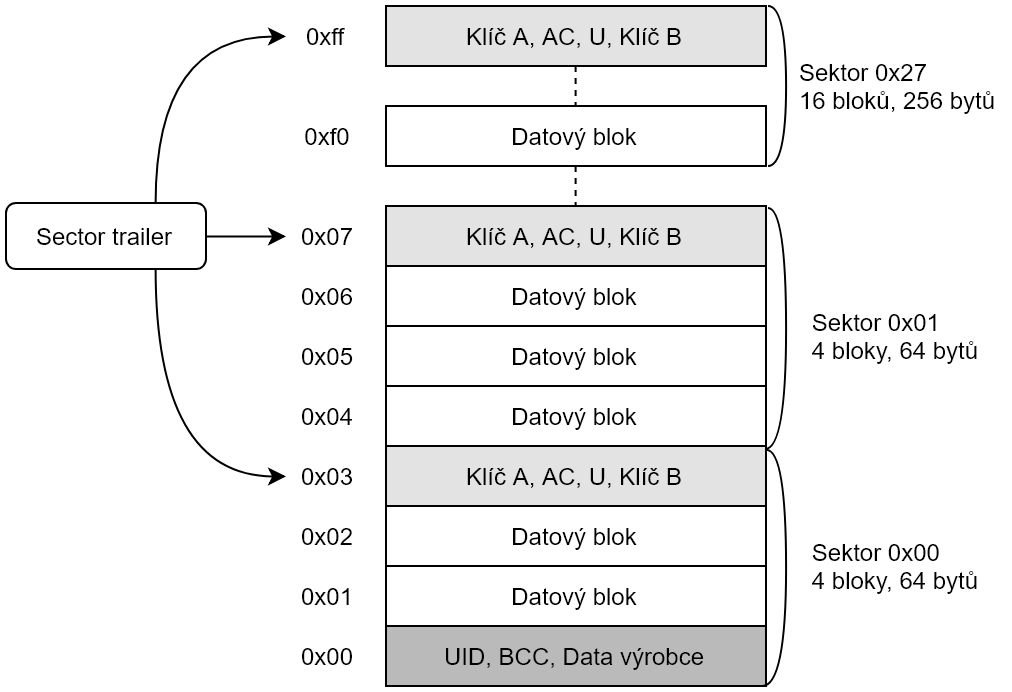
\includegraphics[width=0.6\linewidth,height=180px]{obrazky-figures/MemoryStructure.png}\\[1pt]  
  \caption{Struktura paměti karty Classic\cite{PracticalAttackOnMIFARE}}    
  \label{obrazekStrukturaPametiKarty}
\end{figure*}

\par
Před jakoukoliv operací nad pamětí karty se čtecí zařízení musí nejprve autentizovat proti sektoru se kterým chce pracovat. Každý sektor uzavírá takzvaný sector trailer, speciální datový blok. Obsahuje tajné klíče~A~a~B, které jsou použity při autentizaci. Operace, které je možné nad sektorem provádět, jsou v podmínkách přístupu~AC. Poslední částí sector traileru je jeden datový byte~U, který nemá definovaný účel. Může však být použit pro uložení dat. Sector trailer má zvláštní  podmínky přístupu. Zatímco klíč~A není čitelný nikdy, klíči~B se čitelnost nastavit může. V takovém případě se jím nedá autentizovat a je považován za uživatelská data. Čitelností klíče je myšlen přístup čtecího zařízení k tomuto datovému prostoru s právy pro čtení, karta samotná je může číst bez problémů\cite{PracticalAttackOnMIFARE}. \par
Nastavení klíčů a podmínek přístupu se provede jednoduchým zápisem dat do sector traileru. Nejmenší jednotka přístupu je však celý blok. Načítání, nebo zápis tedy přečte, respektive přepíše blok celý. Změna jediného bytu vyžaduje načtení a~přepsání celého bloku. Pro sector trailer je tato operace o~něco složitější. Čtení bytů na pozicích, kde jsou uloženy klíče, vrací nuly. Tedy změna konfigurace beze změny klíčů vyžaduje znalost těchto klíčů. Takže například nelze zjistit neznámý klíč B změnou konfigurace podmínek přístupu~AC a jeho následným přečtením, protože změna AC vyžaduje přepsání celého bloku i s klíčem\cite{makingTheBestOf}.
\par
Na datových blocích jsou uložena libovolná data, nebo jsou konfigurovány jako blok s hodnotou (value block). Při použití hodnotového bloku je 4bytová, podepsaná hodnota uložena dohromady třikrát. Dvakrát normálně a jednou invertovaně, tedy se všemi bity negovanými. Tyto 4~byty mají uložen nejvýznamnější byte vpravo a nejméně významný vlevo ({little-endian}). Na posledních čtyřech bytech je uložena jedno bytová adresa bloku, která může být použita jako ukazatel. Adresa je uložena čtyři krát po sobě, z toho druhý a čtvrtý byte jsou opět negovány\cite{PracticalAttackOnMIFARE}.

\begin{figure*}[ht]\centering
  \centering
  \hspace*{-0.07\linewidth}
  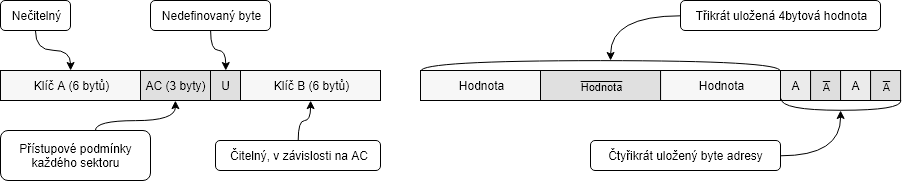
\includegraphics[width=\linewidth]{obrazky-figures/LogicalStructureBetter.png}\\[1pt]  
  \caption{Struktura paměti sector traileru a bloku s hodnotou\cite{PracticalAttackOnMIFARE}}    
  \label{obrazekStrukturaSpecialnichBloku}
\end{figure*}

% subsection struktura_paměti (end)

\subsection{CRYPTO1}
Po autentizaci je veškerá komunikace mezi čtecím zařízením a kartou šifrována. Pro šifrování se používá proprietární proudová šifra CRYPTO1 navržena přímo firmou~NXP\cite{Mifare_Classic_story}. Proudové šifry jsou symetrické šifry kde je důvěrný text neznámé délky (anglicky plaintext) bit po bitu kombinován s proudem pseudonáhodných šifrovacích bitů (dále jen anglicky keystream). Kombinace se nejčastěji provádí pomocí funkce~XOR a jejím výsledkem je zašifrovaný text (cipher text). Šifrovaný text je dešifrován stejnou funkcí a keystreamem. Keystream i důvěrný text musí být stejně dlouhé. Aby bylo možné tohoto dosáhnout s konečnou pamětí, je potřeba keystream generovat. To se děje na základě klíče (anglicky secret key) v generátoru\cite{Stream_ciphers}. Šifra CRYPTO1 jako generátor používá 48bitový posuvný registr s lineární zpětnou vazbou (dále jen LFSR, z anglického Linear Feedback Shift-register) s generačním polynomem~\ref{generatingPolynomial}. Každou periodu hodinového signálu se z dvaceti určitých bitů pomocí filtrační funkce~\ref{filterFunction} vypočítá bit keystreamu, a potom se všechny bity registru posunou doleva. Nejlevější bit je zahozen a nový, pravý bit je jako zpětná vazba vypočítán funkcí~\ref{feedbackFunction}, kde x je aktuální stav registru. V průběhu inicializace se bere v úvahu také vstupní bit, který je kombinován funkcí XOR s~\ref{feedbackFunction}. \cite{Dismantling_Mifare_Classic}.

\begin{multline}
    \label{generatingPolynomial}
    g(x) = x^{48} + x^{43} + x^{39} + x^{38} + x^{36} + x^{34} + x^{33} + x^{31} + x^{29} + x^{24} + \\
     x^{23} + x^{21} + x^{19} + x^{13} + x^{9} + x^{7} + x^{6} + x^{5} + 1  % generating polynomial z dismantling
\end{multline}
\begin{multline}
    \label{feedbackFunction}
    L(x_0, x_1 \dots x_{47}) = x_{0} \oplus x_{5} \oplus x_{9} \oplus x_{10} \oplus x_{12} \oplus x_{14} \oplus x_{15} \oplus x_{17} \oplus x_{19} \oplus x_{24} \oplus \\ 
    x_{25} \oplus x_{27} \oplus x_{29} \oplus x_{35} \oplus x_{39} \oplus x_{41} \oplus x_{42} \oplus x_{43}
\end{multline}
\begin{multline}
    \label{filterFunction}
    f(x_0, x_1 \dots x_{47}) = f_c(f_a(x_{9},x_{11},x_{13},x_{15}),
                               f_b(x_{17},x_{19},x_{21},x_{23}),
                               f_b(x_{25},x_{27},x_{29},x_{31}), \\
                               f_a(x_{33},x_{35},x_{37},x_{39}),
                               f_b(x_{41},x_{43},x_{45},x_{47}))
\end{multline}
\begin{multline}
    \label{filterFunctionC}
    f_c(y_0,y_1,y_2,y_3,y_4) = 
    (y_0 \lor ((y_1 \lor y_4) \land (y_3 \oplus y_4))) \oplus \\
    ((y_0 \oplus(y_1 \land y_3)) \land ((y_2 \oplus y_3) \lor (y_1\land y_4)))
\end{multline}
\begin{equation}
    \label{filterFunctionA}
    f_a(y_0,y_1,y_2,y_3) = 
    ((y_0 \lor y_1) \oplus (y_0 \land y_3)) \oplus (y_2 \land ((y_0 \oplus y_1) \lor y_3))
\end{equation}
\begin{equation}
    \label{filterFunctionB}
    f_b(y_0,y_1,y_2,y_3) = ((y_0 \land y_1) \lor y_2) \oplus ((y_0 \oplus y_1) \land (y_2 \lor y_3))
\end{equation}

\begin{figure*}[ht]\centering
  \centering
  \hspace*{-0.08\linewidth}
  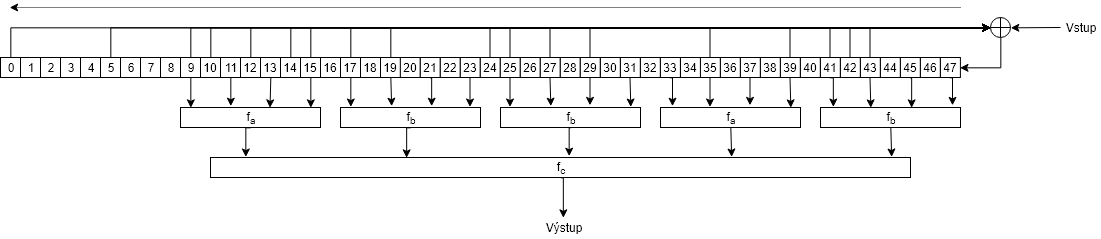
\includegraphics[width=\linewidth]{obrazky-figures/StrukturaSifry.png}\\[1pt]  
  \caption{Struktura šifry CRYPTO1\cite{Wirelessly_Pickpocketing}}    
  \label{obrazekStrukturaSifry}
\end{figure*}

\par
Inicializace šifry probíhá při autentizaci karty a čtecího zařízení. Poté co karta odešle výzvu $n_T$ (viz \ref{autentizace}) je do registru šifry obou zařízení načten sdílený, tajný klíč K. Zde přichází na řadu vstupní bit, který se v tomto momentu vypočítá jako $i = n_T \oplus uid$. Všech 32 bitů tohoto vztahu se naplní do registru spolu s bity zpětné vazby LFSR. Následně se vstupní bity změní na bity výzvy čtecího zařízení $n_R$ a jsou aplikovány stejným způsobem, tedy $g(x) \plus i$. Protože šifrování komunikace začíná při odesílání $n_R$, dřívější bity $n_R$ ovlivňují šifrování pozdějších bitů $n_R$. Na diagramu \ref{obrazekInicializaceSifry} je znázorněna incializace šifry na obou zařízeních. Jediný rozdíl je v tom, že čtecí zařízení nejprve vygeneruje $n_R$ a poté spočítá ${\{n_R\} = n_R \oplus ks}$, zatímco karta přijme $\{n_R\}$ a teprve spočítá $n_R$. Od této chvíle je inicializace hotová a vstupní bit šifry není nadále potřeba\cite{Dismantling_Mifare_Classic}.

\begin{figure*}[ht]\centering
  \centering
  \hspace*{-0.08\linewidth}
  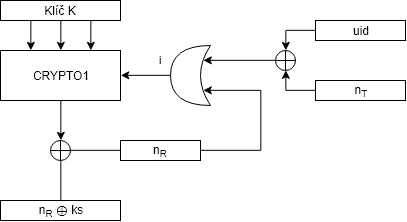
\includegraphics[width=\linewidth]{obrazky-figures/cryptoInitialization.png}\\[1pt]  
  \caption{Diagram inicializace šifry CRYPTO1, kde ks je šifrovací proud (keystream)\cite{Dismantling_Mifare_Classic}}    
  \label{obrazekInicializaceSifry}
\end{figure*}

\subsection{Autentizace}
\label{autentizace}
Komunikace karet MIFARE Classic implementuje standard ISO~14443. Ve čtvrté části se implementace od standardu liší a MIFARE zde používá svůj vlastní, neveřejný protokol. Po vstupu do blízkosti čtecího zařízení a nabití karty nastává antikolizní fáze (viz \ref{obrazekZacatekKomunikace}). Komunikaci zahajuje čtecí zařízení příkazem Select. Odešle \emph{0x93 20}, na což karta odpoví svým~UID~\emph{u}. Čtecí zařízení pošle \emph{0x93~70} následováno~UID vybrané karty a dvěma byty~CRC. Antikolizní fáze je ukončena odpovědí karty~SAK (z anglického Select acknowledge). Nyní je karta v aktivním stavu a připravena přijímat příkazy vyšší vrstvy\cite{PracticalAttackOnMIFARE}.
\par
Čtecí zařízení požádá o autentizaci pro specifický blok odesláním požadavku \emph{0x~60~00~F5~7B}. První byte \emph{0x60} znamená, že se má autentizace provést s klíčem A. Pro autentizaci s klíčem B musí být byte \emph{0x61}. Druhým bytem se vybere blok, pro který se chce čtecí zařízení autentizovat. Blok~0 je v sektoru~0, autentizace tedy proběhne pro celý sektor~0. Pokud by byl požadován například blok~5, autentizace proběhne pro sektor~1. Zbývající dva byty jsou opět CRC\cite{PracticalAttackOnMIFARE}. 
\par
Na tento požadavek karta pošle výzvu (anglicky challenge)~${n_T}$\footnotemark ve formě takzvané nonce\cite{Wirelessly_Pickpocketing}. Nonce je anglický výraz pro slovo na jedno použití. V kryptografii označuje náhodné číslo použité při komunikaci pouze jednou\cite{Nonce_Based_Encryption}. Od této chvíle je komunikace šifrována, tedy XORována s pseudonáhodným proudem bitů (anglicky keystream). Čtecí zařízení odpoví se svou vlastní výzvou~${n_R}$ a odpovědí na výzvu karty~${a_R = suc^{64}(n_T)}$. Autentizace je dokončena odpovědí karty~${a_T = suc^{96}(n_R)}$. Po této odpovědi jsou karta i čtecí zařízení vůči sobě autentizovány. Autentizace je platná pouze pro sektor o který bylo požádáno\cite{Wirelessly_Pickpocketing}. 

\footnotetext{Notace je zachována stejná jako v \cite{Wirelessly_Pickpocketing}, tedy \emph{T} jako tag, \emph{R} jako reader, \emph{n} jako nonce a \emph{a} jako answer}

\begin{figure*}[ht]\centering
  \centering
  \hspace*{-0.08\linewidth}
  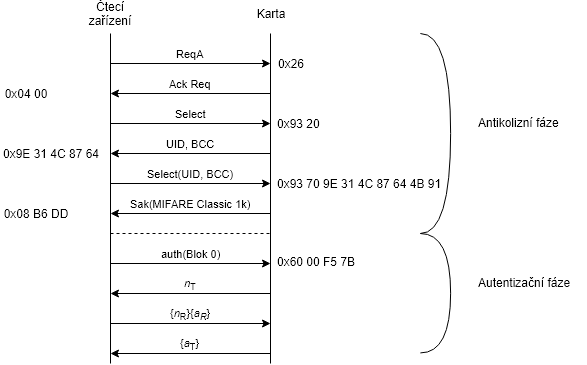
\includegraphics[width=\linewidth]{obrazky-figures/commDiagram.png}\\[1pt]  
  \caption{Antikolizní a autentizační fáze komunikace. Šifrované zprávy jsou ve složených závorkách.\cite{Dismantling_Mifare_Classic}}    
  \label{obrazekZacatekKomunikace}
\end{figure*}

\subsection{Komunikační protokol}
\label{komunikacni_protokol}
\par
Pro manipulaci s daty mají karty Classic malou sadu příkazů. Aby mohly být provedeny nad datovým blokem, musí být čtecí zařízení autentizováno pro sektor, který tento blok obsahuje. Před každým použitím jakéhokoliv příkazu se kontrolují přístupové podmínky. Ne všechny příkazy mohou být povoleny. Například blok může být nastaven pouze pro čtení nebo jiný blok s hodnotou může být pouze inkrementován\cite{PracticalAttackOnMIFARE}.\par
Po autentizaci následuje šifrovaná komunikace s kartou. Příkazy Read a Write čtou, či zapisují jeden blok. Ten může být jak datový, tak hodnotový. Příkaz Write může být použit k formátování datového bloku na blok s hodnotou, nebo na zapsání libovolných dat do bloku. Další příkazy jsou povoleny pouze na hodnotových blocích. Jsou to Decrement, Increment, Restore a Transfer. Příkazy Increment a Decrement inkrementují, nebo dekrementují hodnotu hodnotového bloku a výsledek vloží do paměťového registru. Příkaz Restore načte do registru hodnotu nezměněnou a příkaz Transfer nahraje hodnotu z registru zpět do stejného, nebo jiného bloku\cite{PracticalAttackOnMIFARE}.

\section{Známé zranitelnosti}
Zabezpečení není silná stránka karet MIFARE Classic. Tato podkapitola obsahuje popis jednotlivých nedostatků. Nedostatečná délka šifrovacích klíčů je první z nich. Následuje předvídatelnost výzev posílaných při autentizaci.
Nejjednodušším útokem na chytré karty je takzvaný replay attack. K provedení je nutné z komunikace zachytit~UID, které posílá karta, a poté toto stejné~UID vysílat. Tento útok lze provést nad systémy, které požadují pouze odeslané~UID. Karty MIFARE Classic jsou složitější. Útoky na ně se zaměřují na chyby nebo zranitelné místa v jejich návrhu\cite{Mifare_Classic_story}.
\par
\subsection{Krátké šifrovací klíče}
Pro šifrování karet se používají 48bitové klíče. Tato délka klíčů je ale příliš malá na to, aby zabránila úspěšnému brute force útoku v dosažitelném čase. Proto bylo zavedeno zpoždění v komunikaci a v autentizaci. Každý pokus by trval 6 milisekund. Díky této kompenzaci by online brute force útok na jeden sektor, prohledávající všech $2^{48}$ možných klíčů, trval více než 44~tisíc let. Odhalení algoritmu šifry CRYPTO1 umožnilo provést offline brute force útok. V takovém případě útočník nemusí komunikovat se zařízením pod útokem. Stačí mu pouze záznam komunikace, tím se eliminuje zavedené zpoždění. V prosinci 2007 Nohl a Plötz uvedli, že zařízení za 100\$ dokáže najít klíč přibližně za týden. Tato doba lze dál zkrátit přidáním paměti\cite{Cryptanalisis}.
\par
\subsection{Předvídatelné výzvy}
\label{predvidatelne_nonce}
Aby mohly kryptografické protokoly poskytovat správné zabezpečení, je pro ně zásadní dostatečný generátor pseudonáhodných čísel. Čísla pro MIFARE Classic generuje 16bitový LFSR. Výzvy $n_T$(nonce, viz. \ref{komunikacni_protokol}) použité při autentizaci jsou ale 32bitové. To znamená, že první polovina $n_T$ určuje její zbytek. Sekvence všech výzev se opakuje každých $2^{16} - 1$ cyklů\cite{Cryptanalisis}. Cyklus generátoru karty je rozdílný od čtecího zařízení. Zatímco karta mění stav každou periodu hodinového signálu, čtecí zařízení aktualizuje stav jen při volání generátoru\cite{Dismantling_Mifare_Classic}. Generátor v kartě se resetuje do původního stavu při každém nastartování karty. Výzva poslaná kartou je tedy podmíněna pouze časem mezi zapnutím elektromagnetického pole k nabití karty a momentem odeslání žádosti o autentizaci. Autentizace je tedy zbavena jakékoliv náhodnosti. \par
Útočník s fyzickým přístupem ke kartě ji může \"přinutit\" k odeslání vždy stejné výzvy. K tomu je potřeba po každém pokusu vypnout elektromagnetické pole (zhruba na 30$\mu$s), aby se vybily všechny kondenzátory, znovu zapnout pole a počkat konstantní čas před odesláním požadavku o autentizaci. Druhý způsob spočívá v čekání mezi opětovným odesláním požadavku přesně stanovený čas \emph{t}. Stav generátoru pseudonáhodných čísel se mění každých 9,44$\mu$s. Na vystřídání všech stavů tak stačí pouze $(2^{16} - 1) * 9,44\mu$s $= 618,650ms$. Velikost výzvy je dvojnásobná oproti LFSR, výsledný čas \emph{t} je tedy poloviční $t = 618,650ms/2 = 309,325ms$ \cite{Wirelessly_Pickpocketing}. V novější verzi karet Classic EV1 je tento nedostatek odstraněn nahrazením generátoru pseudonáhodných čísel generátorem náhodných čísel\cite{MIFARE_Classic_Official_about}.

\subsection{Paritní bity}
\label{paritni_bity}
Další slabinou karet MIFARE Classic je jejich řešení paritních bitů. Podle standardu ISO 14443 musí každý odeslaný byte následovat lichý paritní bit. Karty Classic sice s každým odeslaným bytem posílají paritní bit, ten je ale vypočítán už z důvěrného textu (plaintext) a ne z textu šifrovaného (ciphertext), který je skutečně posílán komunikační vrstvou. Kromě toho, odeslané paritní bity jsou šifrovány stejným šifrovacím bitem (keystream), který je použit pro šifrování dalšího bitu plaintextu (viz \ref{parityDiagram})\cite{Cryptanalisis}.
Díky tomuto je s každým odeslaným bytem vyzrazena jednobitová informace o důvěrném textu\cite{Dismantling_Mifare_Classic}. 
\begin{figure*}[ht]\centering
  \centering
  \hspace*{-0.08\linewidth}
  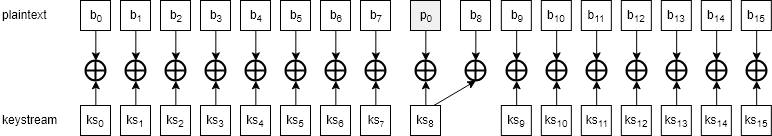
\includegraphics[width=\linewidth]{obrazky-figures/parityBits.png}\\[1pt]  
  \caption{Šifrování paritních bitů \cite{Cryptanalisis}}   
  \label{parityDiagram}
\end{figure*}
\par
V souvislosti s paritními bity existuje ještě jedna slabina. V průběhu autentizační fáze karta vždy nejprve kontroluje právě paritní bity. Když karta přijme $\{n_R\}\{a_R\}$ (viz. \ref{autentizace}) a nějaký z osmi paritních bitů je špatný, karta neodešle žádnou odpověď. V případě, že jsou všechny paritní bity správné, ale $a_R$ je špatně, karta odešle 4bitovou chybovou zprávu $0x5$ indikující selhání autentizace. Jak bylo řečeno v \ref{autentizace}, komunikace je v tuto chvíli šifrována. Ikdyž se čtecí zařízení úspěšně neautentizovalo, dostane chybovou zprávu zašifrovanou. Nelze předpokládat, že si ji správně rozšifruje a dozví se, že došlo k selhání.
Jelikož je kód této chyby známý, lze z šifrované zprávy získat 4 bity keystreamu. Přestože se takovýto únik nemusí zdát jako velký problém, je nepostradatelnou částí mnoha útoků, které cílí na klíče těchto karet.
\par
Jestliže se čtecí zařízení nemá jak dozvědět o selhání při autentizaci, je jedno jestli dostane zprávu šifrovanou, nebo žádnou. Zmíněná slabina tedy lze odstranit vydáním nových karet, které při autentizaci neposílají žádné chybové kódy. Tato metoda je sice nákladná pro již zavedené systémy s kartami v oběhu, ale je pořád kompatibilní s MIFARE Classic protokolem\cite{Cryptanalisis}. 

\subsection{Navrácení stavu posuvného registru}
Stav posuvného registru na začátku inicializace obsahuje tajný klíč sektoru. V průběhu autentizace a šifrování se stav tohoto registru mění. Pokud by se útočníkovi podařil nějakým způsobem získat stav registru v určitém čase a záznam komunikace, lze jednotlivé změny stavu obrátit a deterministicky spočítat jakýkoliv předchozí stav registru včetně tajného klíče. 


\subsection{Vnořená autentizace}
Za předpokladu, že útočník zná a je už ověřen vůči nějakému bloku karty, autentizace vůči dalším blokům probíhá trochu jinak než první. Další autentizaci zahájí útočník odesláním požadavku o autentizaci šifrovaný původním klíčem předchozího bloku. Po zpracování požadavku je vnitřní stav šifry CRYPTO1 nastaven na klíč nového sektoru a autentizační protokol popsaný v \ref{autentizace} začíná od začátku (ovšem bez antikolizní fáze). Změna nastává při odesílání výzvy $n_T$. Ta je totiž nyní odeslána zašifrovaná s tím, že pro šifrování byl použit již nový klíč. Se znalostí šifrování paritních bitů z \ref{paritni_bity} je možné zredukovat $2^16$ výzev na pouhých 64. Kvůli implementaci slabého pseudonáhodného generátoru čísel lze téměř s jistotou určit, která výzva je ta správná. Odeslaná výzva závisí na takzvané vzdálenosti od předchozího pokusu o autentizaci. Tato vzdálenost byla popsána v \cite{Dismantling_Mifare_Classic} jako počet posunutí registru generátoru čísel. Pomocí odhadnuté výzvy lze odhalit 32 bitů šifrovacích bitů (keystream)\cite{Dismantling_Mifare_Classic}.
Tuto slabinu využívají útoky popsané v \cite{Cryptanalisis} a v \cite{Wirelessly_Pickpocketing} kde je útok nazván vnořeným útokem (nested attack).

%Smart Card Security \cite{Smart_Cards_Tokens_Security}{ - str. 224-254}


%                               NADPIS                      
\chapter{Zařízení Chameleon Mini}
\label{zarizeni_chameleon_mini}







\chapter{Závěr}
\label{zaver}


%===============================================================================

  
  % Kompilace po částech (viz výše, nutno odkomentovat)
  % Compilation piecewise (see above, it is necessary to uncomment it)
  %\subfile{projekt-01-uvod-introduction}
  % ...
  %\subfile{chapters/projekt-05-conclusion}


  % Pouzita literatura / Bibliography
  % ----------------------------------------------
\ifslovak
  \makeatletter
  \def\@openbib@code{\addcontentsline{toc}{chapter}{Literatúra}}
  \makeatother
  \bibliographystyle{bib-styles/slovakiso}
\else
  \ifczech
    \makeatletter
    \def\@openbib@code{\addcontentsline{toc}{chapter}{Literatura}}
    \makeatother
    \bibliographystyle{bib-styles/czechiso}
  \else 
    \makeatletter
    \def\@openbib@code{\addcontentsline{toc}{chapter}{Bibliography}}
    \makeatother
    \bibliographystyle{bib-styles/englishiso}
  %  \bibliographystyle{alpha}
  \fi
\fi
  \begin{flushleft}
  \bibliography{projekt-20-literatura-bibliography}
  \end{flushleft}

  % vynechani stranky v oboustrannem rezimu
  % Skip the page in the two-sided mode
  \iftwoside
    \cleardoublepage
  \fi

  % Prilohy / Appendices
  % ---------------------------------------------
  \appendix
\ifczech
  \renewcommand{\appendixpagename}{Přílohy}
  \renewcommand{\appendixtocname}{Přílohy}
  \renewcommand{\appendixname}{Příloha}
\fi
\ifslovak
  \renewcommand{\appendixpagename}{Prílohy}
  \renewcommand{\appendixtocname}{Prílohy}
  \renewcommand{\appendixname}{Príloha}
\fi
%  \appendixpage

% vynechani stranky v oboustrannem rezimu
% Skip the page in the two-sided mode
%\iftwoside
%  \cleardoublepage
%\fi
  
\ifslovak
%  \section*{Zoznam príloh}
%  \addcontentsline{toc}{section}{Zoznam príloh}
\else
  \ifczech
%    \section*{Seznam příloh}
%    \addcontentsline{toc}{section}{Seznam příloh}
  \else
%    \section*{List of Appendices}
%    \addcontentsline{toc}{section}{List of Appendices}
  \fi
\fi
  \startcontents[chapters]
  \setlength{\parskip}{0pt}
  % seznam příloh / list of appendices
  % \printcontents[chapters]{l}{0}{\setcounter{tocdepth}{2}}
  
  \ifODSAZ
    \setlength{\parskip}{0.5\bigskipamount}
  \else
    \setlength{\parskip}{0pt}
  \fi
  
  % vynechani stranky v oboustrannem rezimu
  \iftwoside
    \cleardoublepage
  \fi
  
  % Přílohy / Appendices
  % Tento soubor nahraďte vlastním souborem s přílohami (nadpisy níže jsou pouze pro příklad)
% This file should be replaced with your file with an appendices (headings below are examples only)

% Umístění obsahu paměťového média do příloh je vhodné konzultovat s vedoucím
% Placing of table of contents of the memory media here should be consulted with a supervisor
%\chapter{Obsah přiloženého paměťového média}

%\chapter{Manuál}

%\chapter{Konfigurační soubor} % Configuration file

%\chapter{RelaxNG Schéma konfiguračního souboru} % Scheme of RelaxNG configuration file

%\chapter{Plakát} % poster

\chapter{Jak pracovat s touto šablonou}
\label{jak}

V této příloze je uveden popis jednotlivých částí šablony, po kterém následuje stručný návod, jak s touto šablonou pracovat. Pokud po jejím přečtení k šabloně budete mít nějaké dotazy, připomínky apod., neváhejte a napište na e-mail sablona@fit.vutbr.cz.

\section*{Popis částí šablony}

Po rozbalení šablony naleznete následující soubory a adresáře:
\begin{DESCRIPTION}
  \item [bib-styles] Styly literatury (viz níže). 
  \item [obrazky-figures] Adresář pro Vaše obrázky. Nyní obsahuje placeholder.pdf (tzv. TODO obrázek, který lze použít jako pomůcku při tvorbě technické zprávy), který se s prací neodevzdává. Název adresáře je vhodné zkrátit, aby byl jen ve zvoleném jazyce.
  \item [template-fig] Obrázky šablony (znak VUT).
  \item [fitthesis.cls] Šablona (definice vzhledu).
  \item [Makefile] Makefile pro překlad, počítání normostran, sbalení apod. (viz níže).
  \item [projekt-01-kapitoly-chapters.tex] Soubor pro Váš text (obsah nahraďte).
  \item [projekt-20-literatura-bibliography.bib] Seznam literatury (viz níže).
  \item [projekt-30-prilohy-appendices.tex] Soubor pro přílohy (obsah nahraďte).
  \item [projekt.tex] Hlavní soubor práce -- definice formálních částí.
\end{DESCRIPTION}

Výchozí styl literatury (czechiso) je od Ing. Martínka, přičemž slovenská a anglická verze (slovakiso a englishiso) jsou jeho překlady s drobnými modifikacemi. Oproti normě jsou v~něm určité odlišnosti, ale na FIT je dlouhodobě akceptován. Alternativně můžete využít styl od Ing. Radima Loskota nebo od Ing. Radka Pyšného\footnote{BP Ing. Radka Pyšného \url{http://www.fit.vutbr.cz/study/DP/BP.php?id=7848}}. Alternativní styly obsahují určitá vylepšení, ale zatím nebyly řádně otestovány větším množstvím uživatelů. Lze je považovat za beta verze pro zájemce, kteří svoji práci chtějí mít dokonalou do detailů a neváhají si nastudovat detaily správného formátování citací, aby si mohli ověřit, že je vysázený výsledek v pořádku.

\begin{samepage}
Makefile kromě překladu do PDF nabízí i další funkce:
\begin{itemize}
  \item přejmenování souborů (viz níže),
  \item počítání normostran,
  \item spuštění vlny pro doplnění nezlomitelných mezer,
  \item sbalení výsledku pro odeslání vedoucímu ke kontrole (zkontrolujte, zda sbalí všechny Vámi přidané soubory, a případně doplňte).
\end{itemize}
\end{samepage}

Nezapomeňte, že vlna neřeší všechny nezlomitelné mezery. Vždy je třeba manuální kontrola, zda na konci řádku nezůstalo něco nevhodného -- viz Internetová jazyková příručka\footnote{Internetová jazyková příručka \url{http://prirucka.ujc.cas.cz/?id=880}}.

\paragraph {Pozor na číslování stránek!} Pokud má obsah 2 strany a na 2. jsou jen \uv{Přílohy} a~\uv{Seznam příloh} (ale žádná příloha tam není), z nějakého důvodu se posune číslování stránek o 1 (obsah \uv{nesedí}). Stejný efekt má, když je na 2. či 3. stránce obsahu jen \uv{Literatura} a~je možné, že tohoto problému lze dosáhnout i jinak. Řešení je několik (od~úpravy obsahu, přes nastavení počítadla až po sofistikovanější metody). \textbf{Před odevzdáním proto vždy překontrolujte číslování stran!}


\section*{Doporučený postup práce se šablonou}

\begin{enumerate}
  \item \textbf{Zkontrolujte, zda máte aktuální verzi šablony.} Máte-li šablonu z předchozího roku, na stránkách fakulty již může být novější verze šablony s~aktualizovanými informacemi, opravenými chybami apod.
  \item \textbf{Zvolte si jazyk}, ve kterém budete psát svoji technickou zprávu (česky, slovensky nebo anglicky) a svoji volbu konzultujte s vedoucím práce (nebyla-li dohodnuta předem). Pokud Vámi zvoleným jazykem technické zprávy není čeština, nastavte příslušný parametr šablony v souboru projekt.tex (např.: \verb|documentclass[english]{fitthesis}| a přeložte prohlášení a poděkování do~angličtiny či slovenštiny.
  \item \textbf{Přejmenujte soubory.} Po rozbalení je v šabloně soubor \texttt{projekt.tex}. Pokud jej přeložíte, vznikne PDF s technickou zprávou pojmenované \texttt{projekt.pdf}. Když vedoucímu více studentů pošle \texttt{projekt.pdf} ke kontrole, musí je pracně přejmenovávat. Proto je vždy vhodné tento soubor přejmenovat tak, aby obsahoval Váš login a (případně zkrácené) téma práce. Vyhněte se však použití mezer, diakritiky a speciálních znaků. Vhodný název může být např.: \uv{\texttt{xlogin00-Cisteni-a-extrakce-textu.tex}}. K přejmenování můžete využít i přiložený Makefile:
\begin{verbatim}
make rename NAME=xlogin00-Cisteni-a-extrakce-textu
\end{verbatim}
  \item Vyplňte požadované položky v souboru, který byl původně pojmenován \texttt{projekt.tex}, tedy typ, rok (odevzdání), název práce, svoje jméno, ústav (dle zadání), tituly a~jméno vedoucího, abstrakt, klíčová slova a další formální náležitosti.
  \item Nahraďte obsah souborů s kapitolami práce, literaturou a přílohami obsahem svojí technické zprávy. Jednotlivé přílohy či kapitoly práce může být výhodné uložit do~samostatných souborů -- rozhodnete-li se pro toto řešení, je doporučeno zachovat konvenci pro názvy souborů, přičemž za číslem bude následovat název kapitoly. 
  \item Nepotřebujete-li přílohy, zakomentujte příslušnou část v \texttt{projekt.tex} a příslušný soubor vyprázdněte či smažte. Nesnažte se prosím vymyslet nějakou neúčelnou přílohu jen proto, aby daný soubor bylo čím naplnit. Vhodnou přílohou může být obsah přiloženého paměťového média.
  \item Zadání, které si stáhnete v PDF z IS FIT (odkaz \uv{Zadání pro vložení do práce} či \uv{Thesis assignment}), uložte do souboru \texttt{zadani.pdf} a povolte jeho vložení do práce parametrem šablony v \texttt{projekt.tex} (\verb|documentclass[zadani]{fitthesis}|).
  \item Nechcete-li odkazy tisknout barevně (tedy červený obsah -- bez konzultace s vedoucím nedoporučuji), budete pro tisk vytvářet druhé PDF s tím, že nastavíte parametr šablony pro tisk: (\verb|documentclass[zadani,print]{fitthesis}|). Budete-li tisknout barevně, místo \texttt{print} použijte parametr \texttt{cprint}. Barevné logo se nesmí tisknout černobíle!
  \item Vzor desek, do kterých bude práce vyvázána, si vygenerujte v informačním systému fakulty u zadání. Pro disertační práci lze zapnout parametrem v šabloně \texttt{cover} (více naleznete v souboru \texttt{fitthesis.cls}).
  \item Nezapomeňte, že zdrojové soubory i (obě verze) PDF musíte odevzdat na CD či jiném médiu přiloženém k technické zprávě.
\end{enumerate}

Obsah práce se generuje standardním příkazem \tt \textbackslash tableofcontents \rm (zahrnut v šabloně). Přílohy jsou v něm uvedeny úmyslně.

\subsection*{Pokyny pro oboustranný tisk}
\begin{itemize}
\item \textbf{Oboustranný tisk je doporučeno konzultovat s vedoucím práce.}
\item Je-li práce tištěna oboustranně a její tloušťka je menší než tloušťka desek, nevypadá to dobře.
\item Zapíná se parametrem šablony: \verb|\documentclass[twoside]{fitthesis}|
\item Po vytištění oboustranného listu zkontrolujte, zda je při prosvícení sazební obrazec na obou stranách na stejné pozici. Méně kvalitní tiskárny s duplexní jednotkou mají často posun o 1--3 mm. Toto může být u některých tiskáren řešitelné tak, že vytisknete nejprve liché stránky, pak je dáte do stejného zásobníku a vytisknete sudé.
\item Za titulním listem, obsahem, literaturou, úvodním listem příloh, seznamem příloh a případnými dalšími seznamy je třeba nechat volnou stránku, aby následující část začínala na liché stránce (\textbackslash cleardoublepage).
\item  Konečný výsledek je nutné pečlivě překontrolovat.
\end{itemize}

\subsection*{Styl odstavců}

Odstavce se zarovnávají do bloku a pro jejich formátování existuje více metod. U papírové literatury je častá metoda s~použitím odstavcové zarážky, kdy se u~jednotlivých odstavců textu odsazuje první řádek odstavce asi o~jeden až dva čtverčíky (vždy o~stejnou, předem zvolenou hodnotu), tedy přibližně o~dvě šířky velkého písmene M základního textu. Poslední řádek předchozího odstavce a~první řádek následujícího odstavce se v~takovém případě neoddělují svislou mezerou. Proklad mezi těmito řádky je stejný jako proklad mezi řádky uvnitř odstavce. \cite{fitWeb} 

Další metodou je odsazení odstavců, které je časté u elektronické sazby textů. První řádek odstavce se při této metodě neodsazuje a mezi odstavce se vkládá vertikální mezera o~velikosti 1/2 řádku. Obě metody lze v kvalifikační práci použít, nicméně často je vhodnější druhá z uvedených metod. Metody není vhodné kombinovat.

Jeden z výše uvedených způsobů je v šabloně nastaven jako výchozí, druhý můžete zvolit parametrem šablony \uv{\tt odsaz\rm }.

\subsection*{Užitečné nástroje}
\label{nastroje}

Následující seznam není výčtem všech využitelných nástrojů. Máte-li vyzkoušený osvědčený nástroj, neváhejte jej využít. Pokud však nevíte, který nástroj si zvolit, můžete zvážit některý z následujících:

\begin{description}
	\item[\href{http://miktex.org/download}{MikTeX}] \LaTeX{} pro Windows -- distribuce s jednoduchou instalací a vynikající automatizací stahování balíčků. MikTex obsahuje i vlastní editor, ale spíše doporučuji TeXstudio.
	\item[\href{http://texstudio.sourceforge.net/}{TeXstudio}] Přenositelné opensource GUI pro \LaTeX{}.  Ctrl+klik umožňuje přepínat mezi zdrojovým textem a PDF. Má integrovanou kontrolu pravopisu\footnote{Českou kontrolu pravopisu lze doinstalovat z \url{https://extensions.openoffice.org/de/project/czech-dictionary-pack-ceske-slovniky-cs-cz}}, zvýraznění syntaxe apod. Pro jeho využití je nejprve potřeba nainstalovat MikTeX případně jinou \LaTeX ovou distribuci.
	\item[\href{http://www.winedt.com/}{WinEdt}] Ve Windows je dobrá kombinace WinEdt + MiKTeX. WinEdt je GUI pro Windows, pro jehož využití je nejprve potřeba nainstalovat \href{http://miktex.org/download}{MikTeX} či \href{http://www.tug.org/texlive/}{TeX Live}. 
	\item[\href{http://kile.sourceforge.net/}{Kile}] Editor pro desktopové prostředí KDE (Linux). Umožňuje živé zobrazení náhledu. Pro jeho využití je potřeba mít nainstalovaný \href{http://www.tug.org/texlive/}{TeX Live} a Okular. 
	\item[\href{http://jabref.sourceforge.net/download.php}{JabRef}] Pěkný a jednoduchý program v Javě pro správu souborů s bibliografií (literaturou). Není potřeba se nic učit -- poskytuje jednoduché okno a formulář pro editaci položek.
	\item[\href{https://inkscape.org/en/download/}{InkScape}] Přenositelný opensource editor vektorové grafiky (SVG i PDF). Vynikající nástroj pro tvorbu obrázků do odborného textu. Jeho ovládnutí je obtížnější, ale výsledky stojí za to.
	\item[\href{https://git-scm.com/}{GIT}] Vynikající pro týmovou spolupráci na projektech, ale může výrazně pomoci i jednomu autorovi. Umožňuje jednoduché verzování, zálohování a přenášení mezi více počítači.
	\item[\href{http://www.overleaf.com/}{Overleaf}] Online nástroj pro \LaTeX{}. Přímo zobrazuje náhled a umožňuje jednoduchou spolupráci (vedoucí může průběžně sledovat psaní práce), vyhledávání ve zdrojovém textu kliknutím do PDF, kontrolu pravopisu apod. Zdarma jej však lze využít pouze s určitými omezeními (někomu stačí na disertaci, jiný na ně může narazit i při psaní bakalářské práce) a pro dlouhé texty je pomalejší. Pro vedoucí má FIT licenci a~v~případě, že student narazí na omezení, je s pomocí vedoucího situace řešitelná.
\end{description}

Pozn.: Overleaf nepoužívá Makefile v šabloně -- aby překlad fungoval, je nutné kliknout pravým tlačítkem na \tt projekt.tex \rm a zvolit \uv{Set as Main File}.

\chapter{Psaní anglického textu}
\label{anglicky}
Tato příloha je převzata ze stránek doc. Černockého \cite{CernockyEnglish}.

Spousta lidí píše zprávy k projektům anglicky (a to je dobře!), ale dělá v nich spoustu zbytečných chyb (a to je špatně). Nejsem angličtinář, ale tento jazyk už nějakých pár let používám k psaní, čtení i komunikaci -- tato příloha obsahuje pár důležitých věcí. Pokud chcete napsat práci nebo článek opravdu 100\,\% dobře, nezbude Vám než si najmout rodilého mluvčího (a to by měl by být trochu technicky zdatný a aspoň trochu rozumět tomu, co píšete, ať to neskončí ještě hůř \ldots).

\section*{Obecně}

\begin{itemize}
  \item{Předtím, než budete sami něco psát, si přečtěte pár anglických technických článků a~zkuste si zapamatovat a získat \uv{obecný pocit}, jak se to píše.}
  \item{Používejte vždy korektor pravopisu -- zabudovaný ve Wordu, nebo v OpenOffice, pokud děláte na Linuxu, tak ISPELL a další (většina editorů pro \LaTeX{} má již kontrolu pravopisu integrovanou).}
  \item{Používejte korektor gramatiky. Nevím, jestli je nějaký dostupný na Linuxu, ale ten ve Wordu celkem slušně funguje a pokud Vám něco zelené podtrhne, je tam většinou opravdu chyba. Můžete do něj nakopírovat i zdrojový text pro \LaTeX{}, opravit, a pak uložit opět jako čistý text. Pokud používáte vim, je tam zabudovaný také a zvládne jak překlepy, tak základní gramatiku. V dokumentu \texttt{diplomka.tex} na první řádek napište: 
  \begin{verbatim}
    % vim:spelllang=en_us:spell
  \end{verbatim}
  (případně \texttt{en\_gb} pro OED angličtinu)
  \textit{Poznámka editora:} Existuje i velmi dobrý online nástroj Grammarly\footnote{\url{https://www.grammarly.com/}}, který je v základní verzi zdarma. 
  }
  \item{Online slovníky jsou dobré, ale nepoužívejte je slepě. Většinou dají více variant a ne každá je správně.}
  \item{\begin{samepage}Na vyhledávání a zjištění, co bude asi správné, můžete použít Google. Např.: nevíte, jak se řekne \uv{výhoda tohoto přístupu}. Slovník na seznam.cz dá asi 10 variant. Napište je postupně do vyhledávání na googlu:
  \begin{verbatim}
    "advantage of this approach" 1100000 hits
    "privilege of this approach" 6 hits
    "facility of this approach"  16 hits
  \end{verbatim}
  Neříkám, že je to 100\,\% správně, ale je to určité vodítko. Toto se dá použít i~na~dohledání správných spojek (třeba \uv{among two cases} nebo \uv{between two cases}?)\end{samepage}}
\end{itemize}
       
\section*{SVOMPT a shoda}

Struktura anglické věty je SVOPMT: SUBJECT VERB OBJECT MANNER PLACE TIME a přes to nejede vlak! Není volná jako v češtině. Jinak to je maximálně v nějaké divadelní hře, kde je potřeba něco zdůraznit. Hlavně podmět tam musí vždycky být, na to se často zapomíná, protože v CZ/SK může být zamlčený nebo nevyjádřený. SVOMPT platí i ve vedlejších větách!
\begin{verbatim}
  BAD: We have shown that is faster than the other function. 
  GOOD: We have shown that it is faster than the other function. 
\end{verbatim}

\noindent Shoda podmětu s přísudkem -- zní to šíleně, ale dělá se v tom spousta chyb. 

\begin{verbatim}
  he has 
  the users have 
  people were 
\end{verbatim}

\section*{Členy}

Členy v angličtině jsou noční můra a téměř nikdo z nás je nedává dobře. Základní pravidlo je, že když je něco určitého, musí předtím být \uv{the}. Členy musí být určitě u těchto spojení:
\begin{verbatim}
  the first, the second, ...
  the last
  the most (třetí stupeň přídavných jmen a príslovcí) ...
  the whole 
  the following 
  the figure, the table. 
  the left, the right - on the left pannel, from the left to the right ... 
\end{verbatim}

\noindent Naopak člen NESMÍ být, pokud používáte přesné označení obrázku, kapitoly, atd.
\begin{verbatim}
  in Figure 3.2
  in Chapter 7
  in Table 6.4
\end{verbatim}

\begin{samepage}
\noindent Pozor na \uv{a} vs. \uv{an}, řídí se to podle výslovnosti a ne podle toho, jak je slovo napsané, takže:
\begin{verbatim}
  an HMM
  an XML
  a universal model
  a user
\end{verbatim}
\end{samepage}

\section*{Slovesa}

Pozor na trpné tvary sloves -- u pravidelných je to většinou bez problémů, u nepravidelných často špatně, typicky
\begin{verbatim}
  packet was sent (ne send)
  approach was chosen (ne choosed)
\end{verbatim}
\noindent \ldots vetšinou to opraví korektor pravopisu, ale někdy ne. 

Pozor na časy, občas je v nich pěkný nepořádek. Pokud něco nějak obecně je, přítomný čas. Pokud jste něco udělali, minulý. Pokud to dalo nějaký výsledek a ten výsledek teď existuje a třeba ho nějak diskutujete, přítomný. Nepoužívejte příliš složité časy jako je předpřítomný a vůbec ne předminulý pokud nevíte přesně, co děláte.
\begin{verbatim}
  JFA is a technique that works for everyone in speaker recognition. 
  We implemented it according to Kenny's recipe in \cite{Kenny}. 
  12000 segments from NIST SRE 2006 were processed. When compared 
  with a GMM baseline, the results are completely bad. 
\end{verbatim}

\section*{Délka vět a struktura}

\begin{itemize}
  \item{Pište kratší věty a souvětí, pokud máte něco na 5 řádku, většinou se to nedá číst.}
  \item{Strukturujte věty pomocí čárek (více než v češtině!), hlavně po úvodu věty, po kterém začíná vlastní věta. Někdy se dává čárka i před \uv{and} (na rozdíl od češtiny)}
\end{itemize}
\begin{verbatim}
  In this chapter, we will investigate ... 
  The first technique did not work, the second did not work as well, 
  and the third one also did not work. 
\end{verbatim}

\section*{Specifika technického textu}

Píšete technicky text, proto nepoužívejte zkratky
\begin{verbatim}
  he's
  gonna
  Petr's working on ...
\end{verbatim}
\noindent a podobně. Jediné, které je tolerované, je \uv{doesn't}, ale neuděláte chybu, když napíšete \uv{does not}. 

\begin{samepage}
\noindent V technických textech se spíš používá trpný rod než činný: 
\begin{verbatim}
  BAD: In this chapter, I describe used programming languages. 
  GOOD: In this chapter, used programming languages are described.
\end{verbatim}
\end{samepage}

Pokud už činný použijete, dává se v technických textech spíše \uv{we}, i když na práci děláte sami. \uv{I}, \uv{my}, atd. se používají pouze tam, kde jde o to zdůraznit, že jde o Vaši osobu, tedy třeba v závěru nebo v popisu \uv{originál claims} v disertaci.

\paragraph{Časté chyby ve slovech}

\begin{itemize}
  \item{Pozor na jeho/její, není to it's, ale its }
  \item{Obrázek není picture, ale figure. }
  \item{Spojka \uv{než} je \uv{than}, ne \uv{then} -- bigger than this, smaller than this \ldots hrozně častá chyba! \uv{Then} je pak, potom.}
\end{itemize}


\chapter{Checklist} 
\label{checklist}
Tento checklist byl převzat ze šablony pro kvalifikační práce, která je k dispozici na blogu prof. Herouta \cite{Herout}, který s laskavým dovolením využil nápadu dr. Szökeho%
\footnote{\url{http://blog.igor.szoke.cz/2017/04/predstartovni-priprava-letu-neni.html}}. 

Velká bezpečnost letecké dopravy stojí z části na tom, že lidé kolem letadel mají \textbf{checklisty} na úplně každý, třeba rutinní a dobře zažitý, postup. Jako pilot strpí to, že bude trochu za blbce a opravdu tužtičkou do seznamu úkonů odškrtá dokonale zvládnuté akce, vytiskněte si a odškrtejte před odevzdáním diplomky i vy tento checklist a vyhněte se tak častým chybám, které by mohly mít až fatální následky na výsledné hodnocení Vaší práce.

\subsubsection*{Struktura}
\begin{checklist}
	\item Už ze samotných názvů a struktury kapitol je patrné, že bylo splněno zadání.
	\item V textu se nevyskytuje kapitola, která by měla méně než čtyři strany (kromě úvodu a závěru). Pokud ano, radil(a) jsem se o tom s vedoucím a ten to schválil.
\end{checklist}

\subsubsection*{Obrázky a grafy}
\begin{checklist}
	\item Všechny obrázky a tabulky byly zkontrolovány a jsou poblíž místa, odkud jsou z textu odkazovány, takže nebude problém je najít.
	\item Všechny obrázky a tabulky mají takový popisek, že celý obrázek dává smysl sám o~sobě, bez čtení dalšího textu. Vůbec nevadí, když má popisek několik řádků.
	\item Pokud je obrázek převzatý, tak je to v popisku zmíněno: \uv{Převzato z [X].}
	\item Písmenka ve všech obrázcích používají font podobné velikosti, jako je okolní text (ani výrazně větší, ani výrazně menší).
	\item Grafy a schémata jsou vektorově (tj. v PDF).
	\item Snímky obrazovky nepoužívají ztrátovou kompresi (jsou v PNG).
	\item Všechny obrázky jsou odkázány z textu.
	\item Grafy mají popsané osy (název osy, jednotky, hodnoty) a podle potřeby mřížku.
\end{checklist}

\subsubsection*{Rovnice}
\begin{checklist}
	\item Identifikátory a jejich indexy v rovnicích jsou jednopísmenné (kromě nečastých zvláštních případů jako $t_\mathrm{max}$).
	\item Rovnice jsou číslovány.
	\item Za (nebo vzácně před) rovnicí jsou vysvětleny všechny proměnné a funkce, které zatím vysvětleny nebyly.
\end{checklist}

\subsubsection*{Citace}
\begin{checklist}
    \item \textbf{Všechny použité zdroje jsou citovány.}
	\item Adresy URL odkazující na služby, projekty, zdroje, github apod. jsou odkazovány pomocí \verb|\footnote{\url{...}}|.
    \item Všechny citace používají správné typy.
	\item Citace mají autora, název, vydavatele (název konference), rok vydání.  Když některá nemá, je to dobře zdůvodněný zvláštní případ a vedoucí to odsouhlasil.
\end{checklist}

\subsubsection*{Typografie}
\begin{checklist}
	\item Žádný řádek nepřetéká přes pravý okraj.
	\item Na konci řádku nikde není jednopísmenná předložka (spraví to nedělitelná mezera $\sim$).
	\item Číslo obrázku, tabulky, rovnice, citace není nikde první na novém řádku (spraví to nedělitelná mezera $\sim$).
	\item Před číselným odkazem na poznámku pod čarou nikde není mezera (to jest vždy takto\footnote{příklad poznámky pod čarou}, nikoliv takto \footnote{jiný příklad poznámky pod čarou}).
\end{checklist}

\subsubsection*{Jazyk}
\begin{checklist}
    \item Použil jsem kontrolu pravopisu a v textu nikde nejsou překlepy.
	\item Nechal jsem si text přečíst od (alespoň) jednoho dalšího člověka, který umí dobře česky / anglicky / slovensky.
	\item V práci psané česky nebo slovensky abstrakt zkontroloval někdo, kdo umí opravdu dobře anglicky.
	\item V textu se nikde nepoužívá druhá mluvnická osoba (vy/ty).
	\item Když se v textu vyskytuje první mluvnická osoba (já, my), vždy se popisuje subjektivní záležitost (\textit{rozhodl jsem se}, \textit{navrhl jsem}, \textit{zaměřil jsem se na}, \textit{zjistil jsem} apod.).
	\item V textu se nikde nepoužívají hovorové výrazy.
	\item V českém či slovenském textu se zbytečně nepoužívají anglické výrazy, které mají ustálené české překlady. Např. slovo \textit{defaultní} se nahradí např. slovem \textit{implicitní} nebo \textit{výchozí}.
\end{checklist}

\subsubsection*{Výsledek na datovém médiu, tj. software}
\begin{checklist}
	\item Mám připravené nepřepisovatelné datové médium 
      \begin{itemize}
	  		\item CD-R,
            \item DVD-R,
            \item DVD+R ve formátu ISO9660 (s rozšířením RockRidge a/nebo Jolliet) nebo UDF,
            \item paměťová karta SD (Secure Digital) ve formátu FAT32 nebo exFAT s nastavenou ochranou proti přepisu.
      \end{itemize}
	\item Pokud je výsledek online (služba, aplikace, \dots), URL je viditelně v úvodu a závěru, aby bylo jasné, kde výsledek hledat.
	\item Na médiu nechybí povinné: 
    	\begin{itemize}
    		\item zdrojové kódy (např. Matlab, C/C++,Python, \dots)
            \item knihovny potřebné pro překlad,
            \item přeložené řešení,
            \item PDF s technickou zprávou (je-li pro tisk 2. verze, tak obě),
            \item zdrojový kód zprávy (\LaTeX), 
    	\end{itemize}
        a případně volitelně po dohodě s vedoucím práce
		\begin{itemize}
			\item relevantní (např. testovací) data, 
            \item demonstrační video,
            \item PDF plakátku,
            \item \dots
		\end{itemize}        
	\item Zdrojové kódy jsou refaktorovány, komentovány a označeny hlavičkou s autorstvím, takže se v nich snadno vyzná i někdo další, než sám autor.
    \item Jakákoliv převzatá část zdrojového kódu je řádně citována -- tedy označena úvodním a v případě převzetí více řádků i ukončovacím komentářem. Komentář obsahuje vše, co vyžaduje licence uvedená na webu (vždy je nutné se ji pokusit najít -- např. Stack Overflow\footnote{\url{https://stackoverflow.blog/2009/06/25/attribution-required/}} má striktní pravidla pro citace).
\end{checklist}

\subsubsection*{Odevzdání}

\begin{checklist}
\item Chci práci (na max. 3 roky) utajit? Pokud ano, nejpozději měsíc před termínem odevzdání práce si podám žádost (v IS), ke které přiložím případné stanovisko firmy, jejíž duševní vlastnictví je třeba chránit.
\item Mám splněný minimální počet normostran textu (lze spočítat pomocí Makefile a~odhadem přičíst obrázky). Pokud jsem těsně pod minimem, konzultoval(a) jsem to s~vedoucím.
\item Pokud chci tisknout oboustranně, konzultoval(a) jsem to s~vedoucím a mám správně nastavenou šablonu. Kapitoly začínají na liché stránce.
\item Technickou zprávu mám v deskách z knihařství (min. 1 výtisk, při utajení oba).
\item Za titulním listem práce je zadání (tzn. mám jej stažené z IS a vložené do šablony).
\item V IS jsou abstrakty a klíčová slova.
\item V IS je PDF práce (s klikatelnými odkazy).
\item Oba výtisky práce jsou podepsané.
\item V jednom (při utajení obou) výtisku práce je paměťové médium, na kterém je fixkou napsaný login (fixku na CD lze zapůjčit v knihovně, na Studijním oddělení nebo až při odevzdání).
\end{checklist}


\chapter{\LaTeX pro začátečníky}
\label{latex}

V této kapitole jsou uvedeny některé často využívané balíčky a příkazy pro \LaTeX{}, které mohou být při tvorbě práce potřeba.

\subsection*{Užitečné balíčky}

Studenti při sazbě textu často řeší stejné problémy. Některé z nich lze vyřešit následujícími balíčky pro \LaTeX:

\begin{itemize}
  \item \verb|amsmath| -- rozšířené možnosti sazby rovnic,
  \item \verb|float, afterpage, placeins| -- úprava umístění obrázků/tabulek (specifikátor \texttt{H}),
  \item \verb|fancyvrb, alltt| -- úpravy vlastností prostředí Verbatim, 
  \item \verb|makecell| -- rozšíření možností tabulek,
  \item \verb|pdflscape, rotating| -- natočení stránky o 90 stupňů (pro obrázek či tabulku),
  \item \verb|hyphenat| -- úpravy dělení slov,
  \item \verb|picture, epic, eepic| -- přímé kreslení obrázků.
\end{itemize}

Některé balíčky jsou využity přímo v šabloně (v dolní části souboru \texttt{fitthesis.cls}). Nahlédnutí do jejich dokumentace může být rovněž velmi užitečné.

Sloupec tabulky zarovnaný vlevo s pevnou šířkou je v šabloně definovaný \uv{L} (používá se jako \uv{p}).

Pro odkazování v rámci textu použijte příkaz \verb|\ref{navesti}|. Podle umístění návěští se bude jednat o~číslo kapitoly, podkapitoly, obrázku, tabulky nebo podobného číslovaného prvku). Pokud chcete odkázat stránku práce, použijte příkaz \verb|pageref{navesti}|. Pro citaci literárního odkazu \verb|\cite{identifikator}|. Pro odkazy na rovnice lze použít příkaz \verb|\eqref{navesti}|.

Znak \,--\, (pomlčka) se V \LaTeX u vkládá jako dvě mínus za sebou: -{}-.

\subsection*{Často využívané příkazy pro \LaTeX{}}
\label{sec:Fragments}

Doporučuji nahlédnout do zdrojového textu této podkapitoly a podívat se, jak jsou následující ukázky vysázeny. Ve zdrojovém textu jsou i pomocné komentáře.

% Sloupec zarovnaný vlevo s pevnou šířkou je v šabloně definovaný "L" (používá se jako p)

Příklad tabulky:
\begin{table}[H]
	\vskip6pt
	\caption{Tabulka hodnocení} 
    \vskip6pt
	\centering
	\begin{tabular}{llr}
		\toprule
		\multicolumn{2}{c}{Jméno} \\
		\cmidrule(r){1-2}
		Jméno & Příjmení & Hodnocení \\
		\midrule
		Jan & Novák & $7.5$ \\
		Petr & Novák & $2$ \\
		\bottomrule
	\end{tabular}
	\label{tab:ExampleTable}
\end{table}

% Ohraničení lze upravit dle potřeby:
% http://latex-community.org/forum/viewtopic.php?f=45&t=24323
% http://tex.stackexchange.com/questions/58163/problem-with-multirow-and-table-cell-borders
% http://tex.stackexchange.com/questions/79369/formatting-table-border-and-text-alignment-in-latex-table

\noindent Příklad rovnice:
\begin{equation}
	\cos^3 \theta =\frac{1}{4}\cos\theta+\frac{3}{4}\cos 3\theta
	\label{eq:rovnice2}
\end{equation}
a dvou horizontálně zarovnaných rovnic: % znak & řídí zarovnání
\begin{align} 
    \label{eq:soustava}
	3x &= 6y + 12 \\
	x &= 2y + 4 
\end{align}

Pokud je třeba rovnici citovat v textu, lze použít příkaz \texttt{\\eqref}. Například na rovnici výše lze odkázat~\eqref{eq:rovnice2}. Pokud chcete srovnat číslo rovnic u soustavy, lze použít prostředí \texttt{split}:
\begin{equation} \label{eq:soustavaSrovnana}
\begin{split}
	3x &= 6y + 12 \\
	x &= 2y + 4
\end{split}
\end{equation}

Matematické symboly ($\alpha$) a výrazy lze umístit i do textu $\cos\pi=-1$ a mohou být i~v~poznámce pod čarou%
\footnote{Vzorec v poznámce pod čarou: $\cos\pi=-1$}.

Obrázek~\ref{sirokyObrazek} ukazuje široký obrázek složený z více menších obrázků. Klasický rastrový obrázek se vkládá tak, jak je vidět na obrázku \ref{keepCalm}.

% Využití \begin{figure*} způsobí, že obrázek zabere celou šířku stránky. Takový obrázek dříve mohl být pouze na začátku stránky, případně na konci s využitím balíčku dblfloatfix (případné [h] se ignorovalo a [H] obrázek odstraní). Nové verze LaTeXu už umí i [h].
\begin{figure*}[h]\centering
  \centering
  
\includegraphics[width=\linewidth,height=1.7in]{obrazky-figures/placeholder.pdf}\\[1pt]
  
\includegraphics[width=0.24\linewidth]{obrazky-figures/placeholder.pdf}\hfill
  
\includegraphics[width=0.24\linewidth]{obrazky-figures/placeholder.pdf}\hfill
  
\includegraphics[width=0.24\linewidth]{obrazky-figures/placeholder.pdf}\hfill
  
\includegraphics[width=0.24\linewidth]{obrazky-figures/placeholder.pdf}
  \caption{\textbf{Široký obrázek.} Obrázek může být složen z více menších obrázků. Chcete-li se na tyto dílčí obrázky odkazovat z textu, využijte balíček \texttt{subcaption}.}
  \label{sirokyObrazek}
\end{figure*}

\begin{figure}[hbt]
	\centering
	
\includegraphics[width=0.3\textwidth]{obrazky-figures/keep-calm.png}
	\caption{Dobrý text je špatným textem, který byl několikrát přepsán. Nebojte se prostě něčím začít.}
	\label{keepCalm}
\end{figure}

Další často využívané příkazy naleznete ve zdrojovém textu ukázkového obsahu této šablony.


  
  % Kompilace po částech (viz výše, nutno odkomentovat)
  % Compilation piecewise (see above, it is necessary to uncomment it)
  %\subfile{projekt-30-prilohy-appendices}
  
\end{document}
